\documentclass{article}
\usepackage{caption}
\usepackage{cancel}
\usepackage{tikz}
\usepackage[fontsize=16pt]{fontsize}

\author{}
\date{}
\title{Addition\\
\vspace{28pt}
\begin{normalsize}Applied Scholastics, Ferndale WA \end{normalsize}}

\begin{document}
\maketitle
\pagebreak
\tableofcontents
\pagebreak

\section{Addition}
Addition is a Latin word which means combining things together into one single amount.\\

\vspace{32pt}
Plus is the Latin word for "more," and in writing addition, the plus sign "+" is used. The "+" is the Latin word "et," which means "and," changed in shape a bit.\\

\vspace{32pt}
You can use a number line to show what is happening. Moving to the right on the line represents adding. Here is $2+3=5$:\\

\begin{center}
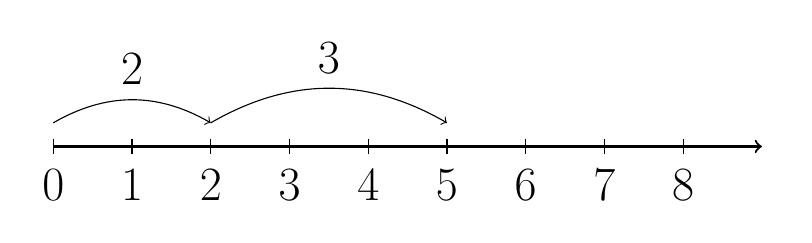
\begin{tikzpicture}
\draw[thick, ->] (0,0) -- (9,0) node[below] {$\ $};
\foreach \n in {0,1,2,3,4,5,6,7,8} {\draw (\n,0.1) -- (\n,-0.1) node[below] {$\n$};}
\draw[->, bend left=30] (0,0.3) to node[above] {$2$} (2,0.3);
\draw[->, bend left=30] (2,0.3) to node[above] {$3$} (5,0.3);
\end{tikzpicture}
\end{center}

\newpage

\vspace{32pt}
The result of addition is called either a sum, which is from Latin meaning "highest," or it is called a total, which is also from Latin meaning "the whole."\\

The first number is called the augend, from Latin meaning "to increase."\\

The number being added to it is the addend, from Latin meaning "put to."\\

{\huge $$\underbrace{2}_{augend} \overbrace{+}^{plus} \underbrace{3}_{addend} = \underbrace{\overbrace{5}^{sum}}_{total}$$}

\newpage

\section{The Addition Table}
Learning addition starts with memorizing the addition of the single digit numbers. You need to know instantly all the sums from 1 + 1 to 9 + 9, and with that known you can add any list of numbers of any size.\\

\begin{table}[h]
\centering
\begin{tabular}{|l|l|l|l|l|l|l|l|l|l|}
\hline
+ & 1  & 2  & 3  & 4  & 5  & 6  & 7  & 8  & 9                       \\ \hline
1 & 2  & 3  & 4  & 5  & 6  & 7  & 8  & 9  & 10                      \\ \hline
2 & 3  & 4  & 5  & 6  & 7  & 8  & 9  & 10 & 11                      \\ \hline
3 & 4  & 5  & 6  & 7  & 8  & 9  & 10 & 11 & 12                      \\ \hline
4 & 5  & 6  & 7  & 8  & 9  & 10 & 11 & 12 & 13                      \\ \hline
5 & 6  & 7  & 8  & 9  & 10 & 11 & 12 & 13 & 14                      \\ \hline
6 & 7  & 8  & 9  & 10 & 11 & 12 & 13 & 14 & 15                      \\ \hline
7 & 8  & 9  & 10 & 11 & 12 & 13 & 14 & 15 & 16                      \\ \hline
8 & 9  & 10 & 11 & 12 & 13 & 14 & 15 & 16 & 17                      \\ \hline
9 & 10 & 11 & 12 & 13 & 14 & 15 & 16 & 17 & \multicolumn{1}{c|}{18} \\ \hline
\end{tabular}
\caption*{The Addition table, which must be memorized}
\end{table}

\newpage

\section{Addition in columns}
Adding multi-digit numbers is done by arranging the numbers into columns aligned at the decimal point. Each column of digits is added separately to get a total.

$72 + 24$ can be solved by $7 + 2 = 9$ and $2 + 4 = 6$ resulting in a sum of 96:

\begin{center}
\begin{tabular}{c@{\,}c@{\,}c@{\,}}
 &7&2\\
+&2&4\\
\hline
=&9&6\\
\hline
\hline
\end{tabular}
\end{center}

The total is separated from the addend and augends by a single line, and is double underlined to indicate that this is a final answer.

Any number of numbers, of any length, can be added in this way, with the units, tens, thousands, and so on all aligned into columns to make the operation clear and simple.\\

\begin{center}
\begin{tabular}{c@{\,}c@{\,}c@{\,}c@{\,}c@{\,}c@{\,}c@{\,}c@{\,}}
 & &1&0&4,&2&1&3\\
 & & & &3,&1&1&2\\
 &1,&2&8&2,&2&3&1\\
+&1,&4&0&0,&3&1&1\\
\hline
=&2,&7&8&9,&8&6&7\\
\hline
\hline
\end{tabular}\\
\end{center}

\newpage

\section{Carrying}
In the case where the total of a column is greater than 9 a series of subtotals must be made that are then added to reach the final sum.\\

\begin{center}
\begin{tabular}{c@{\,}c@{\,}c@{\,}c@{\,}c}
     &1,&2&3&4\\
     &3,&4&5&6\\
   + & &7&8&9\\
\hline
     & & &1&9\\
     & & 1&6&\\
     & 1& 3&&\\
     & 4& & &\\
\hline
     &5,&4&7&9\\
\hline
\hline
\end{tabular}\\
\end{center}

\vspace{28pt}
This use of partial totals is usually abbreviated by "carrying" any tens digit of a partial product over to the column to the left.\\

\begin{center}
\begin{tabular}{c@{\,}c@{\,}c@{\,}c@{\,}c}
	&1,&2&3&4\\
	&3,&4&5&6\\
  + & &7&8&9\\
	&\tiny{1}&\tiny{1}&\tiny{1}&\\
	\hline
	&5,&4&7&9\\
	\hline
	\hline
\end{tabular}
\end{center}

\newpage

\section{Estimation}
It is sometimes not necessary to arrive at an exact sum. If you have a column of numbers you can start with the left-most column and get that subtotal as an estimate of the total for practical purposes, and add in more columns to the right only if that extra precision becomes necessary.

\begin{center}
\begin{tabular}{c@{\,}c@{\,}c@{\,}c@{\,}c}
	&1,&2&3&4\\
	&3,&4&5&6\\
	+ & &7&8&9\\
	\hline
	& 1& &&\\
	& 4& & &\\
	\hline
	&5,&0&0&0\\
	\hline
	\hline
\end{tabular}\\
\end{center}

\newpage

\section{Checking your sum}
After a long addition you may want to sure you have arrived at the correct some without error. If you just repeat the same addition process you may just make the same mistake again so it is better to do the addition a second time but in a different order.\\

Either add the subtotals starting at the right-hand column instead of from the left, or add the augend and addends from the bottom to the top this time.

\newpage

\section{Digit sums}
If an addition is correct, then if you add the digits of the augend and the addends, and the digits of the sum, and keep adding the digits of each result until you get only a single digit for each, then the two "digit sums" will be the same.

Digit sums are not an absolute guarantee of correctness because the different numbers can have the same digit sums, such as 1234 and 3214, but it is still a useful quick check. If the digit sums don't match then you know there is an error somewhere.

\begin{center}
\begin{tabular}{c@{\,}c@{\,}c@{\,}c@{\,}c}
	&1,&2&3&4\\
	&3,&4&5&6\\
  + & &7&8&9\\
	&\tiny{1}&\tiny{1}&\tiny{1}&\\
	\hline
	&5,&4&7&9\\
	\hline
	\hline
\end{tabular}
\end{center}

\vspace{14pt}

\begin{tabular}{c@{\,}c@{\,}c@{\,}c@{\,}c@{\,}c@{\,}c@{\,}c@{\,}c@{\,}cc@{\,}c@{\,}c@{\,}c@{\,}c@{\,}cc@{\,}c@{\,}c@{\,}c@{\,}c@{\,}c@{\,}c@{\,}cc@{\,}c@{\,}c@{\,}c@{\,}c@{\,}}
1&+&2&+&3&+&4&=&10&;&1&+&0&=&1&&&&&&&&&&&&&&\\
3&+&4&+&5&+&6&=&18&;&1&+&8&=&9&&&&&&&&&&&&&&\\
&&7&+&8&+&9&=&24&;&2&+&4&=&6&;&1&+&9&+&6&=&16&;&1&+&6&=&7\\
\hline
\\
5&+&4&+&7&+&9&=&25&;&2&+&5&=&7&&&&&&&&&&&&&&\\
\cline{1-15}
\end{tabular}

\vspace{14pt}
Both digit sums are 7 so you can be pretty sure that the sum is correct.

\newpage

\subsection*{Casting Out 9s}
Adding up digit sums can be simplified by the fact that adding 9 to a number doesn't change it's digit sum.\\

For example, the digit sum of 1234 is 1 + 2 + 3 + 4 = 10; 1 + 0 = 1, and the digit sum of 1234 + 9 = 1243 is 1, and the digit sum of 1243 + 9 = 1252 is also 1.\\

This rule is true for any number, so in calculating digit sums you can disregard any 9s that occur and still get the right digit sum. A digit sum of 9 is equivalent to a digit sum of 0 and that can also be cancelled out.\\

Also, you can cancel out and disregard any two smaller numbers that also add to 9.

\newpage

Say you want to check

\begin{center}
\begin{tabular}{r@{\,}c@{\,}c@{\,}c@{\,}c}
	&1&2&3&4\\
	&2&3&4&5\\
    &3&4&5&6\\
  + &4&5&6&7\\
	&\tiny{1}&\tiny{2}&\tiny{2}&\\
	\hline
 = 1&1,&6&0&2\\
	\hline
	\hline
\end{tabular}\\
\end{center}

Instead of doing 1 + 2 + 3 + 4 = 10 and 1 + 0 = 1, simply cancel any 9s, and cancel any digits that add up to 9, and add up what's left:\\

1234 becomes 1\cancel{234} and the digit sum is 1.

\vspace{7pt}
2345 becomes 23\cancel{45} and the digit sum is 2 + 3 = 5, instead of 2+3+4+5 and 1 + 4 = 5.

\vspace{7pt}
3456 becomes \cancel{3}\cancel{45}\cancel{6} and the digit sum is 0, instead of 3 + 4 + 5 + 6 = 18 and 1 + 8 = \cancel{9}, which can also be cancelled, to equaL 0.

\vspace{7pt}
+ 4567 becomes +\cancel{45}67	and the digit sum is 6 + 7 = 13 and 1 + 3 = 4, instead of 4 + 5 + 6 + 7 = 22 and 2 + 2 = 4.

\vspace{7pt}
= 11,602 becomes =1\cancel{1,602} and the digit sum is 1, instead of 1 + 1 + 6 + 0 + 2 = 1.

\vspace{7pt}
Adding the digit sums of 1 + 5 + 0 + 4 = 10 = 1, which matches the digit sum of the total, we are assured that the sum is correct.
\
\newpage
\
\newpage
\
\newpage
\
\newpage
\

\begin{center}
\linespread{2}\large

Enquiries

\textbf{Applied Scholastics Ferndale}

Principal: Paula McLennan

mobile phone: 0431 683 306

email address: apsferndale@gmail.com

website: apsferndale.webs.com
\end{center}

\end{document}
